\documentclass[a4paper]{article}

\usepackage[margin=1in]{geometry}
\setlength\parindent{0pt}

\usepackage{mathtools}
\usepackage{enumitem} % enumeration label options
\usepackage{amsfonts} % \mathbb, ...
\usepackage{amsthm}
\usepackage{tikz}
\usepackage{caption}
\usepackage{subcaption}

\newtheorem*{theorem}{Theorem}
\newtheorem*{proposition}{Proposition}

\theoremstyle{remark}
\newtheorem*{remark}{Remark}
\newtheorem*{definition}{Definition}
\newtheorem*{example}{Example}
\newtheorem*{notation}{Notation}

\DeclareMathOperator{\ch}{char}

\newcommand{\divides}{\bigm|}

\renewcommand{\P}{\mathbb{P}}
\renewcommand{\O}{\mathcal{O}}
\newcommand{\E}{\mathcal{E}}
\newcommand{\F}{\mathbb{F}}
\newcommand{\N}{\mathbb{N}}
\newcommand{\Z}{\mathbb{Z}}
\newcommand{\Q}{\mathbb{Q}}
\newcommand{\R}{\mathbb{R}}
\newcommand{\C}{\mathbb{C}}

\title{Notes for ``Elliptic Curves'' by Vladimir Dokchitser}
\author{Calum Crossley}
\date{2023-2024}

\begin{document}

\maketitle

Preparatory information:
\begin{itemize}
    \item Books: Silverman's ``Arithmetic of Elliptic Curves''
    \item Prerequisites: basics of Galois theory, basics of number fields, basics of algebraic curves, complex analysis, $p$-adic numbers
    \item Exercise sheets: 1 per lecture, 2 out of 5 exercises for assessment
    \item Lectures: 10 of them
\end{itemize}

Tentative lecture topics:
\begin{enumerate}[label=\arabic*)]
    \item The group law
    \item Geometry over $\C$
    \item Heights
    \item The Mordell-Weil theorem
    \item Geometry over $\Q_p$
    \item Formal groups
    \item Explicit 2-descent
    \item Tate modules
    \item $L$-functions and BSD
    \item Selmer groups
\end{enumerate}

\paragraph{Pre-waffle}

This is a number theory course, so we care about solving Diophantine equations.
For example, what are the rational solutions of $x^2+y^2=1$?
\begin{equation*}
    x = \frac{2t}{t^2+1}, \quad y = \frac{t^2-1}{t^2+1}, \quad t\in\Q.
\end{equation*}
The general case is impossibly hard; it is formally undecidable. We will focus
on curves, such as one equation with two variables. Life is strongly affected by
the geometry over $\C$, where the curve is a closed orientable surface in
projective space.
\begin{itemize}
    \item Genus 0: The Riemann sphere; $\P^1$. The number theory is easy; either
        there are no $\Q$-solutions or infinitely many nicely parametrized, and
        we can decide which (Hasse principle).

    \item Genus 1 (this course): The torus. There can be no $\Q$-solutions, or
        finitely many, or infinitely many. No proven algorithm exists for the
        general case, although there are algorithms conditional on the
        Tate--Shafarevich conjecture or the BSD conjecture.

    \item Genus $\ge2$: There are finitely many $\Q$-solutions by a theorem of
        Faltings.
\end{itemize}

\begin{remark}
    By Siegel's theorem there are only finitely many $\Z$-solutions for $g\ge1$.
\end{remark}

\section{Group Law}

\begin{definition}
    An \emph{elliptic curve} over a field $K$ is a projective non-singular curve
    $E$ of genus 1 over $K$, together with a given $K$-rational point $\O$.
\end{definition}

\begin{example}
    Take $E:y^2=x^3-x$, that is $Y^2Z=X^3-XZ^2$, with $\O=[0:1:0]$ the
    point at infinity.
\end{example}

\begin{definition}
    A \emph{(generalized) Weierstrass equation} over $K$ is an equation of the
    form
    \begin{equation*}
        Y^2Z + a_1XYZ + a_3YZ^2 = X^3 + a_2X^2Z + a_4XZ^2 + a_6Z^3
    \end{equation*}
    with $a_i\in K$. For ease of notation we identify this with the affine
    equation
    \begin{equation*}
        y^2 + a_1xy + a_3y = x^3 + a_2x^2 + a_4x + a_6.
    \end{equation*}
\end{definition}

\begin{remark}
    At infinity we have the point $[0:1:0]$ and no others. This is the standard
    choice for $\O$. If $E$ is non-singular, the genus is 1.
\end{remark}

\begin{notation}
    We write
    \begin{align*}
        E(K)
            &= \{\text{solutions $[X:Y:Z]$ to the equation over $K$}\} \\
            &= \{\O\}\cup\{\text{solutions $(x,y)$ to the equation over $K$}\}.
    \end{align*}
\end{notation}

\begin{example}
    If $E:y^2=f(x)$ with $f(x)$ a monic cubic, then $E(\R)$ looks as follows:
    \begin{figure}[htb]
        \centering
        \begin{subfigure}{0.25\textwidth}
            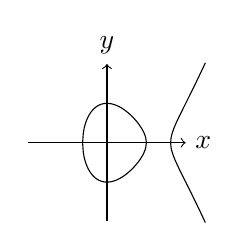
\begin{tikzpicture}
                \draw[->]
                    (-1,0) -- (1,0) node[right] {$x$};
                \draw[->]
                    (0,-1) -- (0,1) node[above] {$y$};
                \draw[scale=0.5,samples=100,domain=-0.618:1,variable=\x]
                    plot ({\x},{sqrt(abs(\x*\x*\x-2*\x*\x+1))});
                \draw[scale=0.5,samples=100,domain=1.618:2.5,variable=\x]
                    plot ({\x},{sqrt(abs(\x*\x*\x-2*\x*\x+1))});
                \draw[scale=0.5,samples=100,domain=-0.618:1,variable=\x]
                    plot ({\x},{-sqrt(abs(\x*\x*\x-2*\x*\x+1))});
                \draw[scale=0.5,samples=100,domain=1.618:2.5,variable=\x]
                    plot ({\x},{-sqrt(abs(\x*\x*\x-2*\x*\x+1))});
            \end{tikzpicture}
        \end{subfigure}
        \begin{subfigure}{0.25\textwidth}
            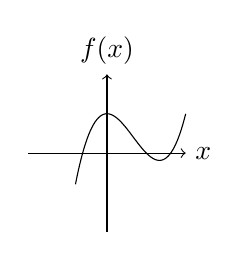
\begin{tikzpicture}
                \draw[->]
                    (-1,0) -- (1,0) node[right] {$x$};
                \draw[->]
                    (0,-1) -- (0,1) node[above] {$f(x)$};
                \draw[scale=0.5,domain=-0.8:2,samples=100,variable=\x]
                    plot ({\x},{\x*\x*\x-2*\x*\x+1});
            \end{tikzpicture}
        \end{subfigure}

        \medskip
        \begin{subfigure}{0.25\textwidth}
            \begin{tikzpicture}
                \draw[->]
                    (-1,0) -- (1,0) node[right] {$x$};
                \draw[->]
                    (0,-1) -- (0,1) node[above] {$y$};
                \draw[scale=0.5,samples=100,domain=1.678:2.5,variable=\x]
                    plot ({\x},{sqrt(abs(\x*\x*\x-1.5*\x*\x-0.5))});
                \draw[scale=0.5,samples=100,domain=1.678:2.5,variable=\x]
                    plot ({\x},{-sqrt(abs(\x*\x*\x-1.5*\x*\x-0.5))});
            \end{tikzpicture}
        \end{subfigure}
        \begin{subfigure}{0.25\textwidth}
            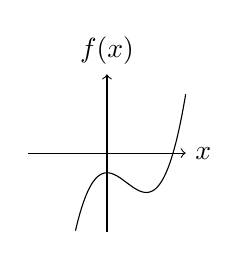
\begin{tikzpicture}
                \draw[->]
                    (-1,0) -- (1,0) node[right] {$x$};
                \draw[->]
                    (0,-1) -- (0,1) node[above] {$f(x)$};
                \draw[scale=0.5,domain=-0.8:2,samples=100,variable=\x]
                    plot ({\x},{\x*\x*\x-1.5*\x*\x-0.5});
            \end{tikzpicture}
        \end{subfigure}

        \medskip
        \begin{subfigure}{0.25\textwidth}
            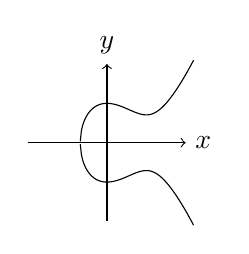
\begin{tikzpicture}
                \draw[->]
                    (-1,0) -- (1,0) node[right] {$x$};
                \draw[->]
                    (0,-1) -- (0,1) node[above] {$y$};
                \draw[scale=0.5,samples=100,domain=-0.678:2.2,variable=\x]
                    plot ({\x},{sqrt(abs(\x*\x*\x-1.5*\x*\x+1))});
                \draw[scale=0.5,samples=100,domain=-0.678:2.2,variable=\x]
                    plot ({\x},{-sqrt(abs(\x*\x*\x-1.5*\x*\x+1))});
            \end{tikzpicture}
        \end{subfigure}
        \begin{subfigure}{0.25\textwidth}
            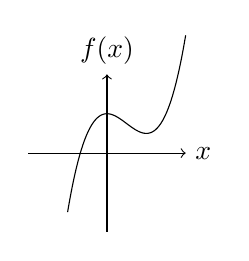
\begin{tikzpicture}
                \draw[->]
                    (-1,0) -- (1,0) node[right] {$x$};
                \draw[->]
                    (0,-1) -- (0,1) node[above] {$f(x)$};
                \draw[scale=0.5,samples=100,domain=-1:2,variable=\x]
                    plot ({\x},{\x*\x*\x-1.5*\x*\x+1});
            \end{tikzpicture}
        \end{subfigure}
    \end{figure}
\end{example}

\begin{theorem}[see Silverman, Chapter III]
    Let $\E$ be an elliptic curve over $K$. Then there exists an isomorphism (of
    projective varieties) from $\E$ to the projective curve defined by
    \begin{equation*}
        E : y^2 + a_1xy + a_3y = x^3 + a_2x^2 + a_4x + a_6
    \end{equation*}
    for some $a_i\in K$, mapping the given $K$-rational point to the point at
    infinity.
\end{theorem}

\begin{remark}
    To keep track of the indices for the Weierstrass equation, give $x$ weight
    2, $y$ weight 3, and $a_i$ weight $i$. The terms all have weight 6.
\end{remark}

\begin{example}
    Take $\E:y^2=x^4-1$ with point $P=(1,0)$.
    \begin{itemize}
        \item Let $x_2=x-1$, giving $y^2=x_2(x_2+2)(x_2^2+2x_2+2)$. (Move $P$ to
            the origin.)
        \item Let $x_3=1/x_2$, giving $(x_3^2y)^2=(1+2x_3)(1+2x_3+2x_3^2)$.
            (Move $P$ to infinity.)
        \item Let $y_2=yx_3^2$, giving $y_2^2=4x_3^3+6x_3^2+4x_3+1$. (Make monic
            in $y$.)
        \item Let $y_3=y_2/2$, giving $y_3^2=x_3^3+\frac{3}{2}x_3^2+x_3+\frac{1}{4}$.
            (Make monic in $x$.)
    \end{itemize}
    Note here we need $\ch K\ne2$. In fact this is a sloppy example, since the
    naive projectivization of the equation is singular. Instead one should
    patch it together with the equation $t^2=1-s^4$ where $s=1/x$, $t=y/x^2$.
\end{example}

\begin{proposition}[see Silverman, Chapter III]
    ~
    \begin{enumerate}[label=(\roman*)]
        \item One can further simplify the Weierstrass equation to
            \begin{equation*}
                E : y^2 = x^3 + ax^2 + bx + c
            \end{equation*}
            when $\ch K\ne2$, and to
            \begin{equation*}
                E : y^2 = x^3 + Ax + B
            \end{equation*}
            when $\ch K\ne2,3$.

        \item Two curves given by generalized Weierstrass equations $E$ and $E'$
            are isomorphic over $K$ iff they are related by a change of
            variables of the form
            \begin{equation*}
                x=u^2x'+r,\quad y=u^3y'+u^2sx'+t
            \end{equation*}
            for some $u,r,s,t\in K$ with $u\ne0$.

        \item If $\ch K\ne2$, and $E:y^2=x^3+ax^2+bx+c$, then $E$ is
            non-singular iff the RHS cubic has no repeated roots, i.e. iff its
            discriminant is non-zero.
    \end{enumerate}
\end{proposition}

\begin{definition}
    Suppose $E/K$ is an elliptic curve given by a Weierstrass equation. Let
    $P,Q\in E(K)$. Define their \emph{sum} $P\oplus Q$ (or just $P+Q$) by the
    following process:
    \begin{figure}[htb]
        \centering
        \begin{tikzpicture}
            \draw[-] (-1.5,-0.9795) -- (2.5,1.039);
            \draw[-] (1.859,2) -- (1.859,-2);
            \node[circle,fill,inner sep=1pt,label=above left:$P$]
                at (-0.544,-0.497) {};
            \node[circle,fill,inner sep=1pt,label=$Q$]
                at (0.94,0.252) {};
            \node[circle,fill,inner sep=1pt,label=below right:$R$]
                at (1.859,0.716) {};
            \node[circle,fill,inner sep=1pt,label=right:$P\oplus Q$]
                at (1.859,-0.716) {};
            \draw[samples=100,domain=-0.618:1,variable=\x]
                plot ({\x},{sqrt(abs(\x*\x*\x-2*\x*\x+1))});
            \draw[samples=100,domain=1.618:3,variable=\x]
                plot ({\x},{sqrt(abs(\x*\x*\x-2*\x*\x+1))});
            \draw[samples=100,domain=-0.618:1,variable=\x]
                plot ({\x},{-sqrt(abs(\x*\x*\x-2*\x*\x+1))});
            \draw[samples=100,domain=1.618:3,variable=\x]
                plot ({\x},{-sqrt(abs(\x*\x*\x-2*\x*\x+1))});
        \end{tikzpicture}
    \end{figure}

    The line through $P$ and $Q$, or the tangent if $P=Q$, meets $E$ at exactly
    one other point $R$ when counting with multiplicity. Repeat the process with
    $\O$ and $R$, i.e. reflect $R$ across $y=0$, to obtain $P\oplus Q$.
\end{definition}

\begin{remark}
    If $P,Q\in E(K)$ then $P\oplus Q\in E(K)$. (If two roots of a cubic are
    rational then the third is too.) This gives a process to construct new
    rational points from old ones.
\end{remark}

\begin{theorem}
    The operation $\oplus$ makes $E(K)$ an abelian group with identity $\O$.
\end{theorem}

\begin{proof}
    See Silverman, Chapter III. See next section for the characteristic 0 case.
\end{proof}

\begin{remark}
    \begin{enumerate}[label=(\roman*)]
        \item If $P=(x_1,y_1)$, then $\ominus P=(x_1,-y_1-a_1x-a_3)$ for a
            generalized Weierstrass equation.

        \item If $F/K$ is a field extension, then $E(K)\subseteq E(F)$ is a
            subgroup.

        \item For $E:y^2=(x-a)(x-b)(x-c)$, the points where $y=0$ are precisely
            the points of order 2.
    \end{enumerate}
\end{remark}

\begin{example}
    The equation $y^2=(x-1)(x-2)(x-3)\mod p$, where $p\ne2$ is prime, has
    total number of solutions $N\equiv3\mod 4$. Indeed $E(\F_p)$ has a subgroup
    isomorphic to $C_2\times C_2$ given by the points of order 2 and the
    identity, so $4\divides\#E(\F_p)$, and removing the point at infinity gives
    $N=\#E(\F_p)-1$.
\end{example}

\begin{theorem}[Mordell 1922]
    Let $E/\Q$ be an elliptic curve. Then $E(\Q)$ is a finitely generated
    abelian group.
\end{theorem}

\begin{proof}
    See section 4.
\end{proof}

\begin{remark}
    So $E(\Q)\cong\Delta\times\Z^r$ for some $r\ge0$ and finite group $\Delta$.
\end{remark}

\begin{definition}
    With $E(\Q)\cong\Delta\times\Z^r$ as above $r$ is the \emph{rank} of
    $E/\Q$, and $\Delta$ the torsion subgroup of $E(\Q)$.
\end{definition}

\begin{remark}
    The result also holds over number fields, and for all abelian varieties
    (Mordell--Weil theorem).
\end{remark}

\begin{remark}
    To describe $E(\Q)$, one is happy with having generators for the group;
    finite data from which the points can be enumerated computationally. One
    cannot parametrize $E(\Q)$ like the conics: there are no non-constant
    $P(t),Q(t)\in\Q(t)$ satisfying the equation of an elliptic curve. (Otherwise
    we get a rational map $\P^1_\C\to E(\C)$ contradicting the Riemann--Hurwitz
    formula.)
\end{remark}

\begin{example}
    ~
    \begin{itemize}
        \item $E:y^2-y=x^3-x$ has
            $E(\Q)=\{\O,(0,0),(0,1),(1,0),(1,1)\}\cong C_5$.

        \item $E:y^2+y=x^3-x$ has $E(\Q)\cong\Z$ generated by $(0,0)$.

        \item $E:y^2+y=x^3+x-2x$ has $E(\Q)\cong\Z^2$ generated by $(0,0)$ and
            $(1,0)$.

        \item $E:y^2=x^3-2x$ has $E(\Q)\cong C_2\times\Z$ generated by $(0,0)$
            and $(-1,1)$ respectively.

        \item $E:y^2=x^3+877x$ has $E(\Q)\cong C_2\times\Z$ generated by $(0,0)$
            and $(\textit{a horrid mess})$ respectively.
    \end{itemize}
\end{example}

\end{document}
